深層学習は,人間の神経細胞の仕組みを模したシステムであるニューラルネットワークがベースになっている\cite{deeplearning}.そして,ニューラルネットワークを多層にして用いることで,データに含まれる特徴を段階的により深く学習することが可能になる.深層学習を行う場合,ラベル付けされたデータが必要になるが,現在はDSTC2\cite{dstc2}やMulti-Woz\cite{multi-woz}など,ユーザの対話状態やシステムの対話行為などをラベル付けした対話データセットが公開されている.このようなデータが公開されたことで,深層学習による対話状態追跡の研究が盛んに行われている.
\par
深層学習による対話状態追跡では,通常発話文を入力として直接対話状態を出力する\cite{nbt,e2e}.対話状態であるインテントや各スロットの値に関してはデータセットによって事前に候補が与えられている.そのため,発話文から得た情報を基にそれぞれの全候補にわたる確率分布を出力し,確率最大のものをインテントあるいはスロット値として選択する.しかし,そのようなモデルは候補として与えられていない値を推測できないため,言語理解などを用いて候補外の値も推定可能にするモデル\cite{joint,trade,mrc}の研究が行われている.そのようなモデルの例として,Rastogi ら\cite{joint} のモデルを図\ref{fig:joint}に示して説明する.
\begin{figure}[t]
  \begin{center}
    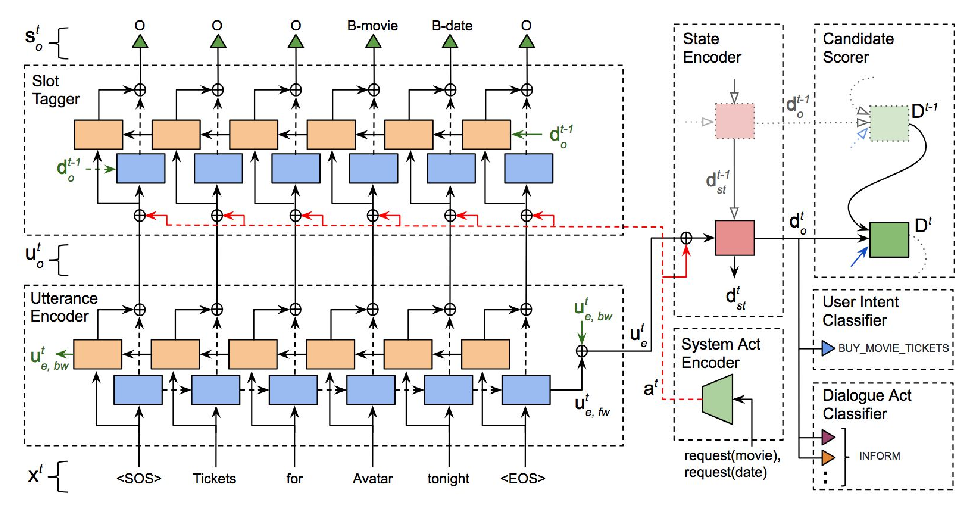
\includegraphics[width=15cm]{chapter2/joint.eps}
    \caption{言語理解と対話状態追跡を共同で学習するモデル\cite{joint}}
    \label{fig:joint}
  \end{center}
\end{figure}
このモデルは,Utterance Encoder, System Act Encoder, State Encoder によってユーザの発話,システムの対話行為,対話状態の特徴量を得る.これら特徴量は言語理解部と対話状態追跡部で共有される.言語理解部である Slot Tagger は発話中の単語ごとにラベルを付けてスロット値の候補となる単語を見つける.ラベルは,スロット値の開始地点を示す B ラベル,スロット値の継続を示す I ラベル,スロット値でないことを示す O ラベルで構成される IOB ラベルが用いられる.B ラベルと I ラベルはスロットの数だけ作成される.Slot Tagger で見つけられたスロット値はスロット値候補リストに追加される.対話状態追跡部は,User Intent Classifierでユーザの目的を推定し,Dialogue Act Classifierでユーザの対話行為を推定し,Candidate Scorer でスロット値候補リスト中の候補のランク付けを行いスロットに値を割り当てる.
\par
言語理解と対話状態追跡を共同で学習することで,言語理解部で発生した誤りが対話状態追跡部に伝搬するのを防ぐことが可能になる.また,言語理解部と対話状態追跡部でエンコーダのネットワーク層を共有できるため,性能の向上とネットワーク層のパラメータの数の削減が同時に行える\cite{joint}.しかし,このようなモデルは新しいドメインに適応させたい場合,言語理解部のIOBラベルを増やして再学習する必要がある.したがって,現在は新しいドメインに再学習なしで適応可能な拡張性のある対話状態追跡の研究が注目されている.